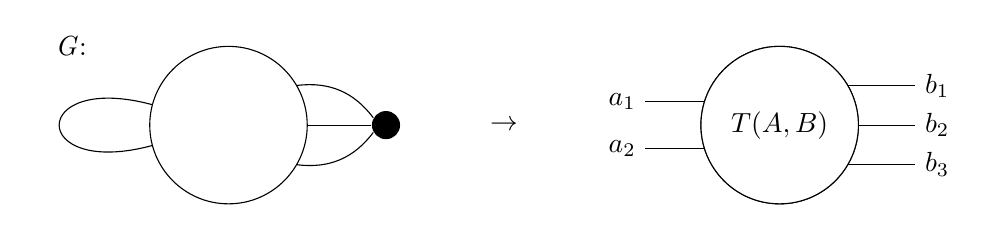
\begin{tikzpicture}[scale=1]
	\tikzset{every loop/.style={}}
	\node[draw=none] (G) at (-2, 1) {\textit{G}:};
	\node[shape=circle,draw=black, minimum size=2cm] (1) at (0,0) {};
	\node[shape=circle,color=black,fill,text width=1pt] (2) at (2,0) {};
	
	\path (1) edge (2);
	\path (1) edge [bend left] (2);
	\path (1) edge [bend right] (2);
	
	\path (1)
	edge (2)
	edge [loop left] node {} ()
	;
	
	\node[draw=none] (arrow) at (3.5, 0) {$\rightarrow$};

	\node[shape=circle,draw=black, minimum size=2cm] (1) at (7,0) {$T(A,B)$};
	\node[shape=rectangle,draw=none] (1mid) at (7,0) {$T(A,B)$};
	\node[draw=none] (2) at (9,0.5) {$b_1$};
	\node[draw=none] (3) at (9,0) {$b_2$};
	\node[draw=none] (4) at (9,-0.5) {$b_3$};
	
	\node[draw=none] (5) at (5,0.3) {$a_1$};
	\node[draw=none] (6) at (5,-0.3) {$a_2$};
	
	\draw (2) -- (2-|1mid.east);
	\draw (3) -- (3-|1mid.east);
	\draw (4) -- (4-|1mid.east);
	
	\draw (5) -- (5-|1mid.west);
	\draw (6) -- (6-|1mid.west);
	
	\node[shape=circle,draw=black,fill=white, minimum size=2cm] (1) at (7,0) {$T(A,B)$};
				
\end{tikzpicture}